\subsection{Process 2: Emergency Handler}
\label{subsec:process_2}
Emergency Handler is the second process which involves the detection and rapid response to emergency situations, typically triggered by the presence of emergency vehicles such as ambulances or fire trucks. In the event that the Traffic Control Unit (TCU) receives a signal from an emergency vehicle, it initiates a swift and high-priority response.
Upon receiving the signal, the TCU processes the information and dynamically adjusts the idle signal scheduling state to transition into an emergency state. This modification ensures that the traffic control system promptly prioritizes and facilitates the smooth passage of the emergency vehicle through the affected area. This feature is pivotal in enhancing the system's responsiveness to critical situations, ultimately contributing to the efficiency of emergency services and the overall safety of the community. Illustrated in Figure 9:
\begin{itemize}
\item 
The Traffic Control Unit (TCU) consistently monitors for input pertaining to the presence of emergency vehicles.
\item Upon receiving input indicating the presence of a high-priority vehicle, the TCU swiftly transitions to an emergency vehicle Right of Way (ROW) state. Simultaneously, the TCU modifies the standard signal scheduling to align with the exigencies of the emergency situation. 
\end{itemize}
\begin{figure}[h]
\centering
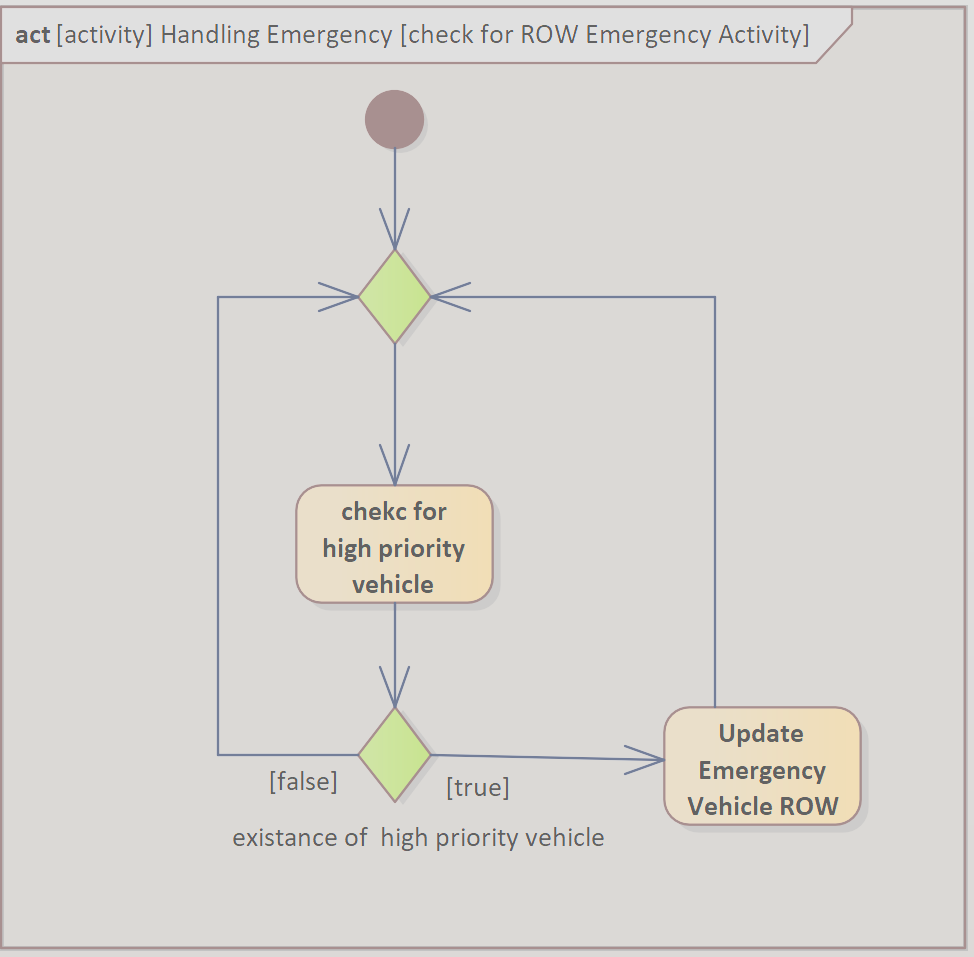
\includegraphics[width=0.5\linewidth]{images/process_2_activity.png}
\caption{\label{fig:process_2_activity}\\Emergency Response Activity}
\end{figure}
The interaction between the emergency vehicle and the Traffic Control Unit (TCU) changes the the idle scheduling within the traffic system. Initiated by the Emergency Listener, the process unfolds as follows: upon receiving input, the Emergency Listener transmits a signal request to the TCU. Subsequently, the TCU engages in processing this signal request, evaluating the decision to be made.
In instances where the existence of the emergency vehicle is determined, the TCU issues a message instructing the adjustment of the signal schedulers behavior. This adjustment is based on the Emergency Vehicle ROW. The interaction between these components is visually depicted in  Figure 10, that contribute to the effective management and optimization of the traffic system.
\begin{figure}[h]
\centering
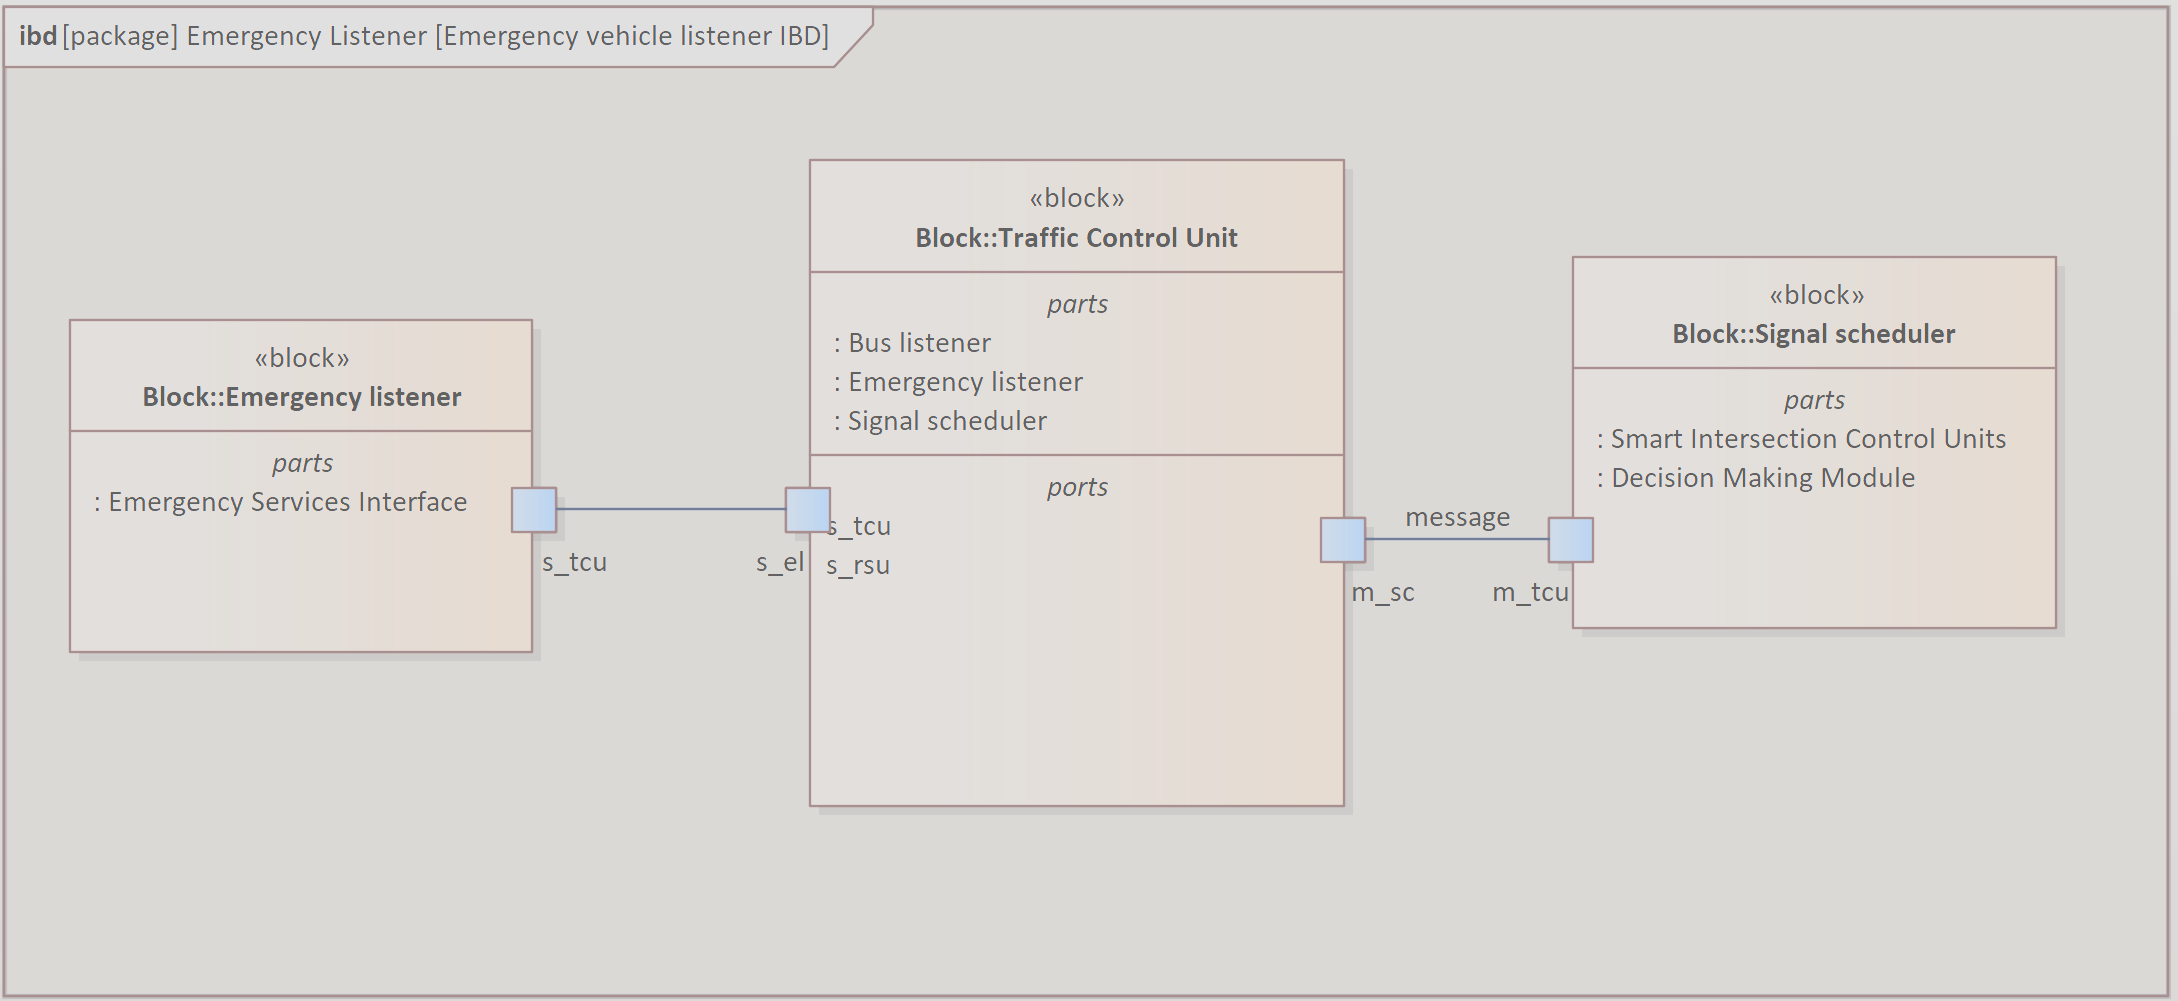
\includegraphics[width=1\linewidth]{images/emergency_listener_ibd.png}
\caption{\label{fig:bus_listeneribd}\\Interaction between Emergency Listener and Signal Scheduler}
\end{figure}